\documentclass{article}
\usepackage{graphicx} % Required for inserting images
\usepackage{float} 

\begin{document}

% Title Page
\title{RASD Document}
\author{Alessandro Salvatore, Erdal Yalçın, Leonardo Ratti}
\date{Academic Year: 2024-25}
\maketitle

% Table of Contents
\newpage
\tableofcontents

% Sections (These are examples, replace with actual content as needed)
\newpage
\section{Introduction}
\subsection{Purpose}
Students\&Companies (S\&C) is a dynamic platform designed to connect university students seeking internships with companies offering valuable opportunities. By leveraging students' skills, experiences, and career interests alongside the specific needs and offerings of companies, S\&C aims to create seamless matches. The platform provides a recommendation system that notifies students about relevant internships and informs companies of suitable candidates. It also facilitates the selection process, supports feedback exchange, and helps both parties refine their profiles for better alignment. S\&C results useful thanks to the offered tools for monitoring internship progress and resolving issues collaboratively.
\subsubsection{Goals}
The goals specify what the platform will allow users to achieve in the real world, everything else will not be allowed. 
\\All the starred words will be defined in section 1.3 to avoid any ambiguity.
\begin{itemize}
  \item \textbf{G1} Allows registered companies* to post* and advertise* the available internships that they offer.
  \item \textbf{G2} Allows registered students* to proactively and autonomously search and apply* to advertised internships.
  \item \textbf{G3} Helps registered students and registered companies by suggesting them appealing templates for their CVs and internship projects drafts.
  \item \textbf{G4} Allows a registered student to be recommended a list of advertised internships that might be of interest to him/her with respect to: his/her uploaded CV, the internships projects* and users'* feedbacks.
  \item \textbf{G5} Allows a registered company to be recommended a list of registered students who might be of interest for one of its advertised internships with respect to: their uploaded CVs, the internship project and users' feedbacks.
  \item \textbf{G6} Allows a registered company to view the list of all the students who applied to one of its advertised internships grouped by the internship they applied to.
  \item \textbf{G7} Allows a company to get in contact* with the candidates* for one of its internships and, only after, manage their selection process*.
  \item \textbf{G8} Allows registered companies and students that are taking part* in an ongoing internship to comment about it.
  \item \textbf{G9} Allows a registered university to view the comments about an ongoing internship, written either by its interning students or by the host company.
  \item \textbf{G10} Allows a registered university to interrupt an ongoing internship involving one its students.
  \item \textbf{G11} Allows companies and students to provide feedback about a past internships only if they respectively offered it and took part in it.

\end{itemize}
\subsection{Scope}
\subsubsection{World Phenomena}
    \begin{itemize}
        \item \textbf{W1} A company wants to advertise an internship. 
        \item \textbf{W2} A student wants to find an internship opportunity.
        \item \textbf{W3} A student wants to discover interesting companies.
        \item \textbf{W4} A company wants to interview the internship candidate and select them.
        \item \textbf{W5} A student wants to evaluate an internship process
        \item \textbf{W6} A company and a student want to improve the internship advertisement and the CV, respectively.
        \item \textbf{W7} A University wants to follow an internship process
    \end{itemize}
\subsubsection{Shared Phenomena}
    \textit{Controlled by World}
    \begin{itemize}
        \item \textbf{S1} A student searches for internships on the platform.
        \item \textbf{S2} A company posts an internship advertisement on the platform.
        \item \textbf{S3} A student selects and accepts internships he wants to make contact with.
        \item \textbf{S4} A company selects and accepts a number between all the interested and recommended students as candidates for the given internship.
        \item \textbf{S5} A Student or a Company sends information of any type about the state of an on-going internship, like complaining or providing general information.
        \item \textbf{S6} A University interrupts an internship of a student after some complaints from the company or from the student. 
        \item \textbf{S7} A user registers either as Student, Company or University.
        
        \item \textbf{S1} A registered student submit their resumes on the S\&C.
        \item \textbf{S2} A registered company advertises an internship opportunity on S\&C.
        \item \textbf{S3} A company selects a student through the S\&C based on interesting skills from the student's CV. 
        \item \textbf{S4} A student selects the internship they want to apply for through the S\&C.
        \item \textbf{S5} A company creates interview request through the S\&C for the interview, after the match.
        \item \textbf{S6} A student and a company are able to provide feedback on their experiences, after the selection process.
        \item \textbf{S7} A company offers an internship position to the relevant student through the S\&C.
        \item \textbf{S8} A student accepts or declines an internship position through the S\&C.
        \item \textbf{S9} A student's university follows up on feedback about the internship process through the S\&C and is able to interrupt the internship if necessary.
        \item \textbf{S10} A student updates their resume based on the suggestions received from the S\&C.
        \item \textbf{S11} A student updates their advertisement based on the suggestions received from the S\&C.
    \end{itemize}
    \textit{Controlled by Machine}
    \begin{itemize}
        \item \textbf{S12} The system notifies a company about an interesting student resume.
        \item \textbf{S13} The system notifies to a student an internship that might interest him is available.
        \item \textbf{S14} The system starts a contact process when both an internship and a student confirm an interest in each other.
        \item \textbf{S15} The system shows some information about a student profiles to a company.
        \item \textbf{S16} The system shows some information about an internship advertisement and a company profile to a student.
        \item \textbf{S17} The system notifies a student when the interview date is scheduled.
        \item \textbf{S18} The system creates an interview link and sends to the both sides.
        \item \textbf{S19} The system analyzes the feedback data and provides suggestions for improving the profiles. 
        \item \textbf{S20} The system recommends interesting profiles and shows to the both sides.
        \item \textbf{S21} The system notifies a student when the company's decision is announced.
        \item \textbf{S22} The system creates a link for following and handling the internship process and sends to the student's university.
        \item \textbf{S23} The system notifies a student when internship is advertised from a favorite company which has manually searched for.
    \end{itemize}
\subsection{Definitions, Acronyms, Abbreviations}

\subsubsection{Definitions}
    \begin{itemize}
        \item Recommendation: It's a platform feature that starts a matching between a company and a student. If both parties accept the recommendation, the student is taken for the selection process
        \item *Accepting: The act of students or companies, who got recommended to each other, to confirm their interest. 
        \item Selection: It's the process that starts after the expiration date of applying for the internship. The company interviews every accepted student and picks the best one(s) for their needs. 
        \item Feedback: Refers to the comments that both parties are asked to write at the end of the internship contract, in order to improve the platform.
        \item Observation: Is anything written in the dedicated Observations section. Serves the student or the company currently engaged, to highlight something about the experience with each other. If that's a complaint from either, the University of the student will manage the situation.
        \item Complaint: It's a specific type of Observation, where the University of the student is called to act and manage the situation between the parties.
        \item Contact: The mutual acceptance between student and company.
    \end{itemize}
\subsubsection{Acronyms}
    \begin{itemize}
        \item S\&C: "Students\&Companies", the name of the platform
    \end{itemize}
\subsubsection{Abbreviations}
    \begin{itemize}
        \item WPn: n-th World Phenomena
        \item SPn: n-th Shared Phenomena
        \item Gn: n-th Goal
        \item Dn: n-th Domain Assumption
        \item Rn: n-th Requirement
    \end{itemize}
\subsection{Revision history}
\subsection{Reference Documents}
    \begin{itemize}
        \item Software Engineering 2 A.Y. 2024/2025 Slides (course material)
        \item Assignment RDD A.Y. 2024/2025 (Requirement Engineering and Design Project: goal, schedule, and rules)
    \end{itemize}

\subsection{Document Structure}

\section{Overall Description}
\subsection{Product Perspective}
\subsubsection{Scenarios}
    \begin{itemize}
        \item 1st Scenario: Signing up. User John has accessed the opening page; he registers into the site as a student, filling the required data and is sent back to the opening page.
        \item 2nd Scenario: Logging in. User John is in the opening page; he logs into the site using his credentials, and can now access to his possible operations.
        \item 3rd Scenario: Finalizing registration. The student John opens his profile page and uploads his CV document into the platform; he studies at Polime, so he connects his university mail with his account.
        \item 4th Scenario: Starting an offer. The company Emazon posts an internship offer on the platform, deciding the expiration date and the duration of it. Then Emazon lists the tasks the student will have to perform, the application domain and other relevant things regarding the internship.  
        \item 5th Scenario: Platform recommendation. Upon CV uploading, the   platform analyzes John's CV and automatically suggests him all the current potential interesting internship offers. After Emazon has posted its internship offer, it gets notified to him too.
        \item 6th Scenario: Searching Internships. John opens the page of the available internships. He filters out the ones without benefits, and is left with few options. He applies for Guggl's offer.
        \item 7th Scenario: Student accepts recommendation. John gets the
        notification from Emazon and decides to accept it.
        \item 8th Scenario: Company accepts students. After Emazon posted the internship offer, it gets recommended some students by the platform, while some other students found the internship by manual searching. Emazon accepts John and some other students.
        \item 9th Scenario: Entering the selection. After the expiration date passes, the company starts the selection process. Emazon proposes the interviews dates and time schedules through the dedicated interface to all the contacted students.
        \item 10th Scenario: Student chooses interview day. Since John has established contact with Emazon, he selects the time and day of the interview through the dedicated interface.
        \item 11th Scenario: Student joins the interview. When the scheduled day for the interview comes, John can meet the interviewer using the link posted by the company on the platform. After some time, the platform officially notifies him that he was selected.
        \item 12th Scenario: Writing Observations. Emazon writes a complaint in the provided space about John's current behaviour.
        \item 13th Scenario: University acts. The University Polime gets a complaint from Emazon about John's behaviour. Polime decides to interrupt his internship.
        \item 14th Scenario: Giving Feedback. At the end of the internship, John and Emazon fill a questionnaire about their experience with the platform and give suggestions to it.
    \end{itemize}
\subsubsection{Class Diagram}
The UML Class Diagram shown below provides a conceptual, high-level representation of the intended software. At this stage, it may include entities that will not necessarily be part of the final system. Additionally, this diagram intentionally omits methods and other detailed elements that will be addressed in the design phase.
\\The three main components are User, Internship and Student\&Company (which represents the software itself). They are connected with arrows in order to recreate the interactions between one another. The User views the Internship according to his granted permissions. Then he/she interacts with the platform (i.e. accepts a recommendation, submits feedback... ) and eventually the system accordingly manages the Internship.
\begin{figure}[H]
    \centering
    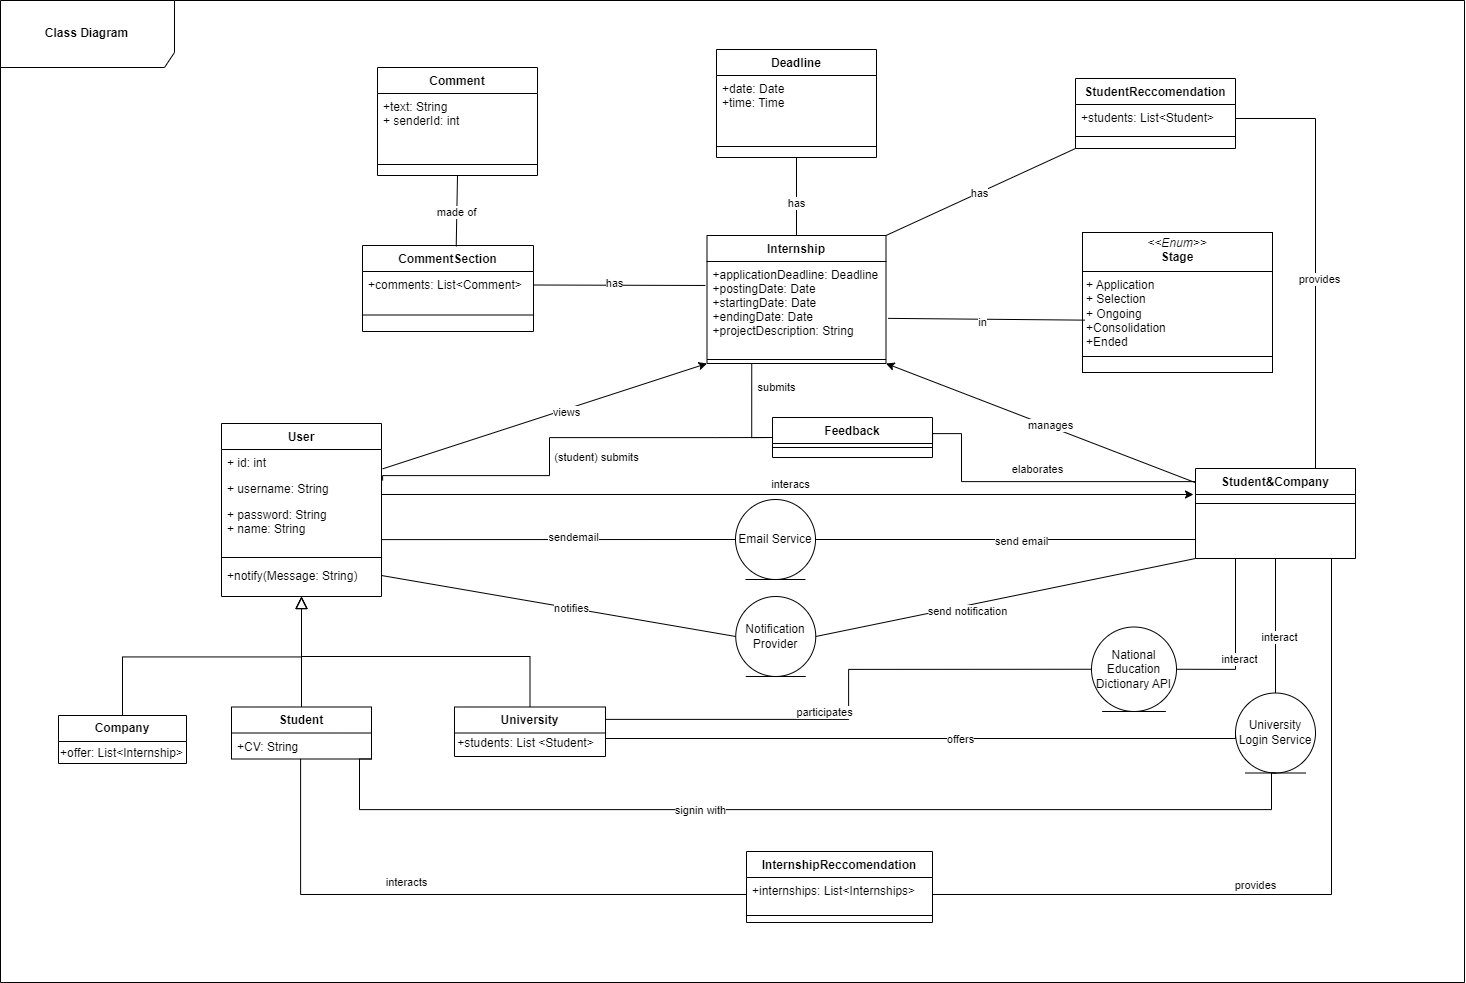
\includegraphics[scale = 0.30]{figures/Class Diagram.drawio.png}
    \centering
\end{figure}
\subsubsection{State Charts}
\subsection{Product Functions}
\subsubsection{Requirements}
    \begin{itemize}
        \item \textbf{Requirement} Students can share their CVs on the platform
        \item \textbf{R1} The system must allow a student who wants to register to sign up.
        \item \textbf{R2} The system must allow a company who wants to register to sign up.
        \item \textbf{R3} The system must allow a university who wants to register to sign up.
        \item \textbf{R4} The system must allow registered users to sign in using their credentials.
        \item \textbf{R5} The system must allow registered users who wishes to reset their password to change it after completing various procedures and checks.
        \item \textbf{R6} The system must be able to send notifications to all users.
        \item \textbf{R7} The system must allow registered students to enter information from their CV to complete their profiles.
        \item \textbf{R8} The system must allow registered companies to post internship advertisements.
        \item \textbf{R9} The system must allow companies to review students' CVs and select candidates who meet their internship requirements.
        \item \textbf{R10} The system must allow students to review internship advertisements and select them if they wish to apply.
         \item \textbf{R11} The system must allow students to manually search for internship opportunities and save them to their favorites.
         \item \textbf{R12} The system must notify students when there are updates regarding the internships at the companies in their favorites that they wish to apply for.
        \item \textbf{R13} The system must match a student and a company that select each other and notify them afterward, but only if a match is done.
        \item \textbf{R14} The system must allow companies to choose a suitable date for the interview, but only after a match is done.
        \item \textbf{R15} The system must schedule an interview at the date and time specified by the company and notify the selected students.
        \item \textbf{R16} The system must recommend a student and a company profile to each other and allow them to review whether the company has an active internship position and if the profiles could attract each other's interest.
        \item \textbf{R17} The system must allow companies to offer internship proposals to selected students after the interview process is completed.
        \item \textbf{R18} The system must allow companies to evaluate students during the internship process and provide feedback on their CVs.
        \item \textbf{R19} The system must allow students to give feedback on their internship experiences.
        \item \textbf{R20} The system must provide suggestions to users for improving their profiles based on feedback.
        \item \textbf{R21} The system must notify students when there are updates regarding the results of the internships they have applied for.
        \item \textbf{R22} The system must allow selected students to accept or decline internship proposal sent by companies.    
         \item \textbf{R23} The system must notify students about deadlines for accepting internship offers.
        \item \textbf{R24} The system must allow companies to view and manage applications for the internships they have posted, including the status of interviews and offers.  
        \item \textbf{R25} The system must allow students to view all details about the internships they have applied for, such as completion status, rejections, and deadlines.
        \item \textbf{R26} The system must send invitations to universities to follow their students' internship progress.
        \item \textbf{R27} The system must allow universities to follow internship process, handle complaints raised by students, and interrupt an internship if necessary, but only if the relevant student's university is signed in.
        \end{itemize}
\subsection{User characteristics}
     A User can be one of three types: Student, University, Company. Each role has access to distinct functionalities and is driven by different motivations.
     \begin{itemize}
        \item Students: They are students of some university; they want to apply for internships, either helped by the recommendations from the platform or by looking for internship themselves. If they have something to say about their on-going internship, they can make observations in the platform.
        \item Companies: They want to recruit students for their internship projects. They are aided in the selection process from the platform. They might want to make observations or complaints about the hired student.
        \item Universities: They want to manage their students' on-going internship, handling their complaints or the ones coming from the company of the internship.     
     \end{itemize}
\subsection{Assumptions, dependencies and constraints}
This section serves as a comprehensive overview of critical factors which must be considered during the implementation of the platform. It consolidates the foundational assumptions made during project planning and highlights eventual dependencies.
\subsubsection{Domain Assumptions}
    \begin{itemize}
        \item D1 The User must have a working Internet connection.
        \item D2 Students are enrolled in universities as student of any kind.
    \end{itemize}
\subsubsection{Dependencies}
An EmailService is needed, because in the registration process a verifcation email must be sent by the system to let Users successfully sign up.\\ \\The system also wants to have some connection with the universities, so a service for that is needed.

\section{Specific Requirements}
\subsection{External Interface Requirements}
\subsubsection{User Interfaces}
\subsubsection{Hardware Interfaces}
\subsubsection{Software Interfaces}
\subsubsection{Communication Interfaces}
\subsection{Functional Requirements}
\subsubsection{Use Case Diagrams}
\begin{figure}[H]
    \centering
    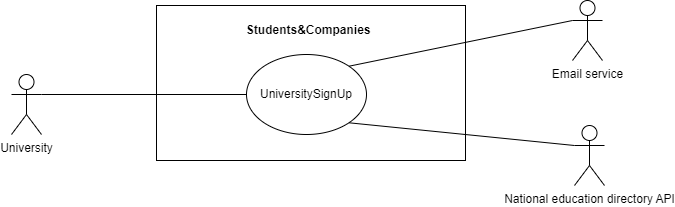
\includegraphics[scale = 0.45]{figures/UniversityLogin.drawio.png}
    \caption{UniversitySignUp}
    \centering
\end{figure}
\begin{figure}[H]
    \centering
    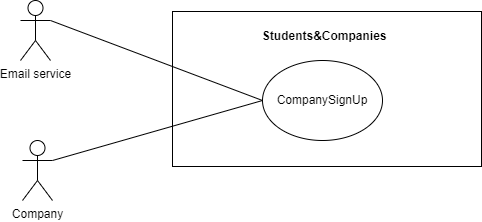
\includegraphics[scale = 0.45]{figures/use_case_1-CompanyLogin.drawio.png}
    \caption{CompanySignUp}
    \centering
\end{figure}
\begin{figure}[H]
    \centering
    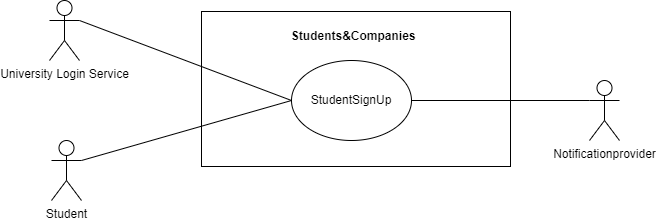
\includegraphics[scale = 0.45]{figures/use_case_1-StudentLogin.drawio.png}
    \caption{StudentLogin}
    \centering
\end{figure}
\begin{figure}[H]
    \centering
    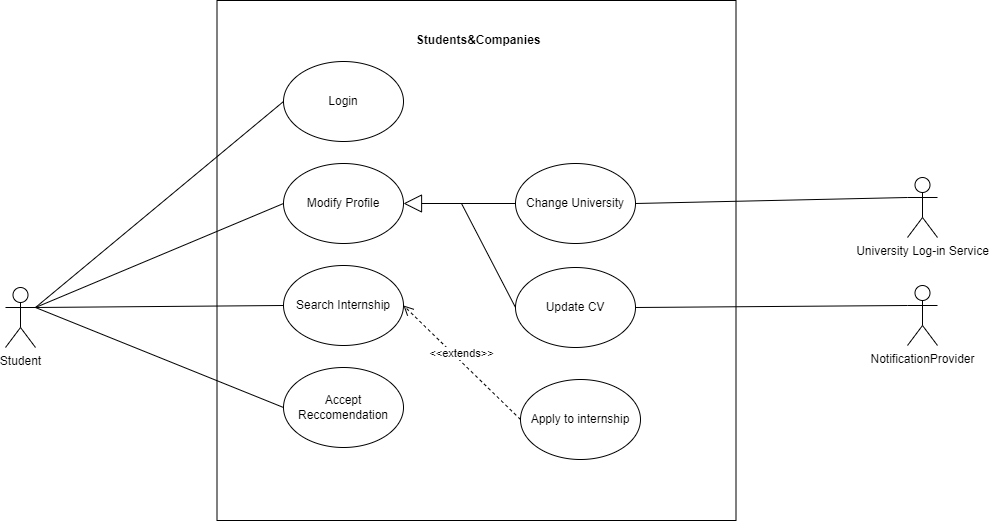
\includegraphics[scale = 0.45]{figures/Student.drawio.png}
    \caption{Student}
    \centering
\end{figure}
\begin{figure}[H]
    \centering
    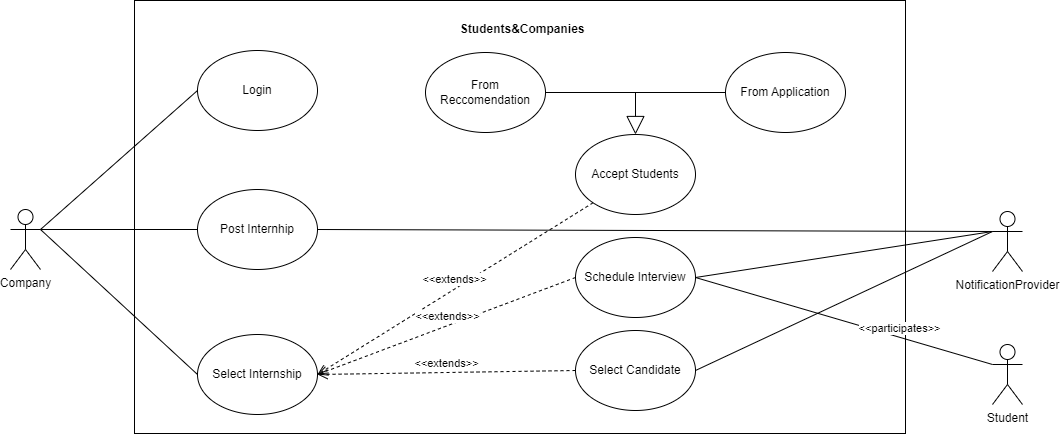
\includegraphics[scale = 0.4]{figures/Company.drawio.png}
    \caption{Company}
    \centering
\end{figure}
\begin{figure}[H]
    \centering
    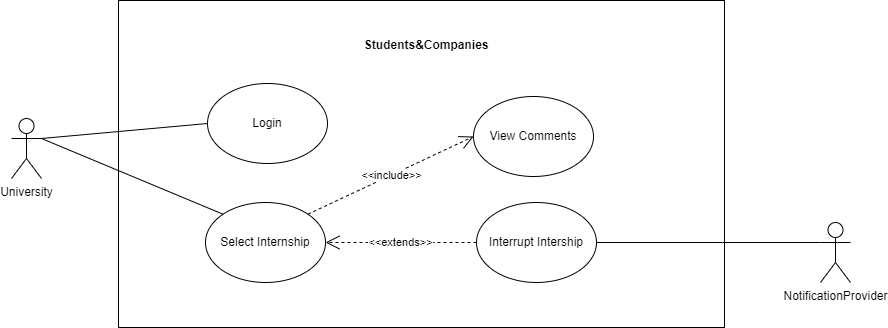
\includegraphics[scale = 0.45]{figures/use_case_1-University.drawio.png}
    \caption{University}
    \centering
\end{figure}
\begin{figure}[H]
    \centering
    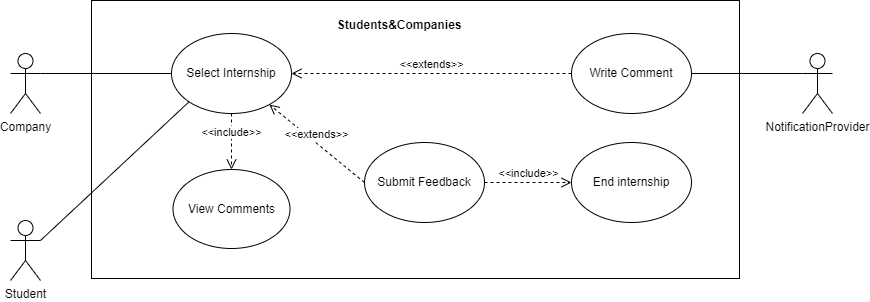
\includegraphics[scale = 0.45]{figures/use_case_1-Student - Company.drawio.png}
    \caption{Internship}
    \centering
\end{figure}
\subsubsection{Use cases}
\subsubsection{mapping}
\subsection{Performance Requirements}
\subsection{Design Constraints}
\subsubsection{Standards compliance}
\subsubsection{Hardware limitations}
\subsection{Software System Attributes}
\subsubsection{Reliability and Availability}
\subsubsection{Security}
\subsubsection{Maintainability}
\subsubsection{Portability}

\section{Formal Analysis Using Alloy}
\subsection{Objectives of the Analysis}
\subsection{Alloy Code}

\section{Effort Spent}
\subsection{Effort Spent per Unit}

\section{References}
\subsection{References and Tools}

\maketitle



\end{document}






